\exercisetitle{
Una línea de transmisión con $Z_0=50 \Omega$ está cargada con una impedancia de $Z_L=50+j35 \Omega$. ¿A qu ́e distancia
de la carga debe colocarse una sección adaptadora en $\lambda/4$ para acoplar la línea a la carga?  ¿Cuál debe
ser el valor de la impedancia característica de la sección $\lambda/4$
}
Se nos pide introducir una línea $\lambda/4$ en el sistema anterior con el fin de adaptar la línea a la carga. Para ello primero debemos encontrar a que distancia de la carga la impedancia se hace puramente real, con lo que podremos aplicar la expresión de una línea  $\lambda/4$.
\begin{figure}[h]
  \centering
  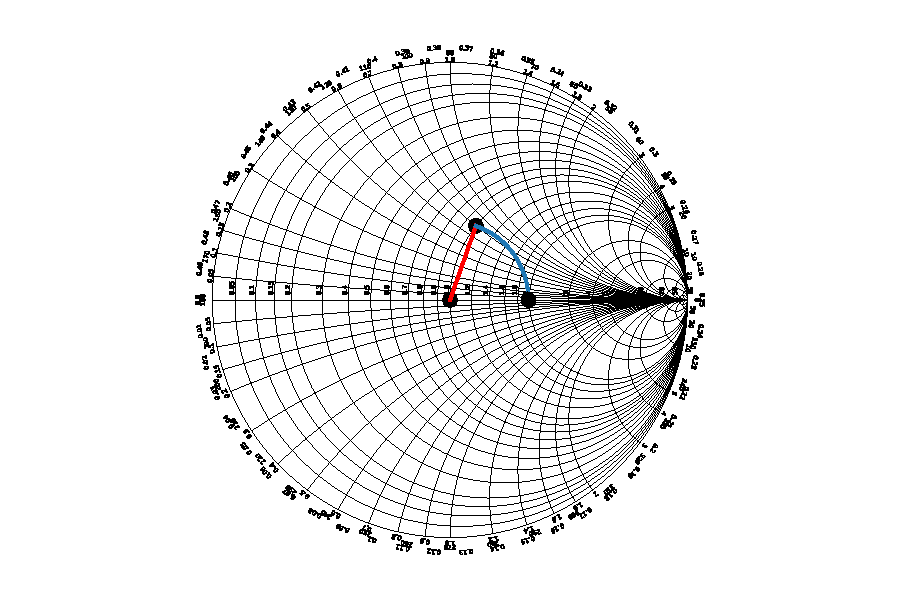
\includegraphics{ej9/images/out.pdf}
  \caption{$z_{in} = a + 0j$}
  \label{ej2smith}
\end{figure}

Donde vemos que $z_{in} = 2$ que tras denormalizar de $50 \Omega$, obtendremos $Z_{in} = 100 \Omega$, con esto ya podemos calcular la impedancia intrínseca de la insercción $\lambda/4$ como:
\[ Z_0 = \sqrt{Z_{in} Z_{Z_L}} = \sqrt{100 \times 50} = 70.7 \Omega \]
